% Author: Izaak Neutelings (September 2021)
% Inspiration:
%   https://jila.colorado.edu/~ajsh/insidebh/penrose.html
%   https://tex.stackexchange.com/questions/99124/how-to-draw-penrose-diagrams-with-tikz
%   coordinates: https://arxiv.org/pdf/physics/0611033.pdf
%   https://arxiv.org/pdf/0711.0873.pdf
\documentclass[border=3pt,tikz]{standalone}
\usepackage{tikz}
\usepackage{amsmath} % for \text
\usepackage{mathrsfs} % for \mathscr
\usepackage{xfp} % higher precision (16 digits?)
\usepackage[outline]{contour} % glow around text
\usetikzlibrary{decorations.markings,decorations.pathmorphing}
\usetikzlibrary{angles,quotes} % for pic (angle labels)
\usetikzlibrary{arrows.meta} % for arrow size
\contourlength{1.4pt}

\newcommand{\calI}{\mathscr{I}} %\mathcal
\tikzset{>=latex} % for LaTeX arrow head
\colorlet{myred}{red!80!black}
\colorlet{myblue}{blue!80!black}
\colorlet{mygreen}{green!80!black}
\colorlet{mydarkred}{red!50!black}
\colorlet{mydarkblue}{blue!50!black}
\colorlet{mylightblue}{mydarkblue!6}
\colorlet{mypurple}{blue!40!red!80!black}
\colorlet{mydarkpurple}{blue!40!red!50!black}
\colorlet{mylightpurple}{mydarkpurple!80!red!6}
\colorlet{myorange}{orange!40!yellow!95!black}
\tikzstyle{cone}=[mydarkblue,line width=0.2,top color=blue!60!black!30,
                  bottom color=blue!60!black!50!red!30,shading angle=60,fill opacity=0.9]
\tikzstyle{cone back}=[mydarkblue,line width=0.1,dash pattern=on 1pt off 1pt]
\tikzstyle{world line}=[myblue!60,line width=0.4]
\tikzstyle{world line t}=[mypurple!60,line width=0.4]
\tikzstyle{particle}=[mygreen,line width=0.5]
\tikzstyle{photon}=[-{Latex[length=4,width=3]},myorange,line width=0.4,decorate,
                    decoration={snake,amplitude=0.9,segment length=4,post length=3.8}]
\tikzstyle{singularity}=[myred,line width=0.6,decorate,
                         decoration={zigzag,amplitude=2,segment length=6.17}]
\tikzset{declare function={%
  penrose(\x,\c)  = {\fpeval{2/pi*atan( (sqrt((1+tan(\x)^2)^2+4*\c*\c*tan(\x)^2)-1-tan(\x)^2) /(2*\c*tan(\x)^2) )}};%
  penroseu(\x,\t) = {\fpeval{atan(\x+\t)/pi+atan(\x-\t)/pi}};%
  penrosev(\x,\t) = {\fpeval{atan(\x+\t)/pi-atan(\x-\t)/pi}};%
  kruskal(\x,\c)  = {\fpeval{asin( \c*sin(2*\x) )*2/pi}};% Penrose coordinates for Kruskal
}}
\def\tick#1#2{\draw[thick] (#1) ++ (#2:0.04) --++ (#2-180:0.08)}
\def\Nsamples{40} % number samples in plot

% LIGHTCONE
\def\R{0.08} % size lightcone
\def\e{0.08} % vertical scale
\def\ang{45} % angle light cone
\def\angb{acos(sqrt(\e)*sin(\ang))} % angle ellipse center to point of tangency
\def\a{\R*sin(\ang)*sqrt(1-\e*sin(\ang)^2)/(1-\e*sin(\ang)^2)} % vertical radius
\def\b{\R*sqrt(\e)*sin(\ang)*cos(\ang)/(1-\e*sin(\ang)^2)} % horizontal radius
\def\coneback#1{ % light cone part to be drawn behind world lines
  \draw[cone back] % dashed line back
    (#1)++(-45:\R) arc({90-\angb}:{90+\angb}:{\a} and {\b});
  \draw[cone,shading angle=-60] % top edge & inside
    (#1)++(0,{\R*cos(\ang)/(1-\e*sin(\ang)^2)}) ellipse({\a} and {\b});
}
\def\conefront#1{ % light cone part to be drawn over world lines
  \draw[cone] % light cone outside
    (#1) --++ (45:\R) arc({\angb-90}:{-90-\angb}:{\a} and {\b})
     --++ (-45:2*\R) arc({90-\angb}:{-270+\angb}:{\a} and {\b}) -- cycle;
}

\begin{document}


% PENROSE DIAGRAM of Minkowski space - 45 rotation
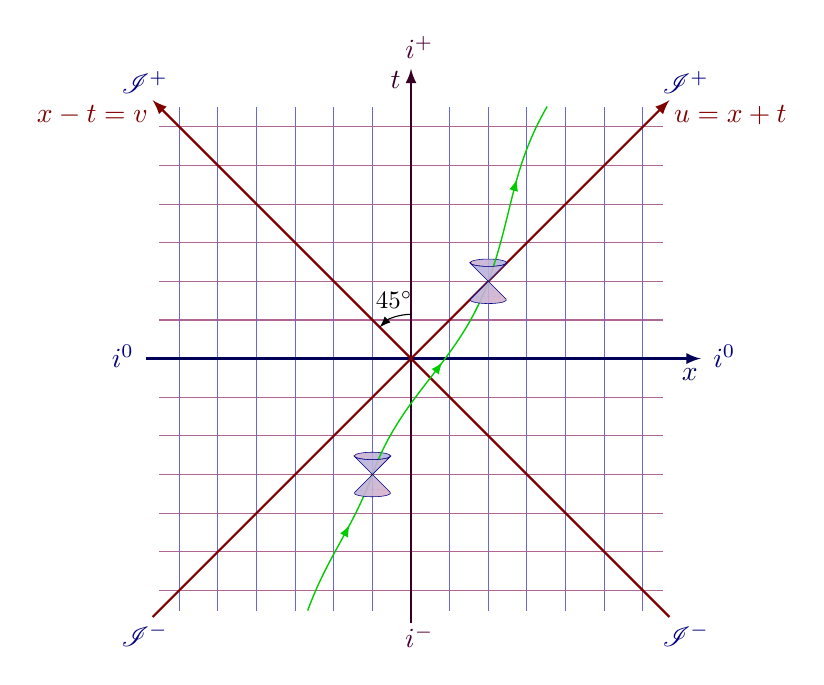
\begin{tikzpicture}[scale=3.2]
  \message{Penrose diagram (45 rotation)^^J}
  
  \def\R{0.10} % size lightcone
  \def\Nlines{6} % number of world lines (at constant r/t)
  \pgfmathsetmacro\d{0.92/\Nlines} % grid size
  
  \coordinate (O) at (0,0);
  \coordinate (W) at (-1.05,0);
  \coordinate (E) at (1.15,0);
  \coordinate (S) at (0,-1.05);
  \coordinate (N) at (0,1.15);
  \coordinate (SW) at (-135:1.45);
  \coordinate (SE) at (-45:1.45);
  \coordinate (NW) at (135:1.45);
  \coordinate (NE) at (45:1.45);
  \coordinate (X0) at (-0.41,-1);
  \coordinate (X1) at (-\d,-3*\d);
  \coordinate (X2) at (2*\d,2*\d);
  \coordinate (X3) at (0.54,1);
  
  % WORLD LINES GRID
  \message{Making world lines...^^J}
  \foreach \i [evaluate={\x=\i*\d;}] in {1,...,\Nlines}{
    \message{  Running i/N=\i/\Nlines, x=\x...^^J}
    \draw[world line]   (-\x,-1) -- (-\x,1);
    \draw[world line]   ( \x,-1) -- ( \x,1);
    \draw[world line t] (-1,-\x) -- (1,-\x);
    \draw[world line t] (-1, \x) -- (1, \x);
  }
  
  % AXES
  \draw[->,thick,mydarkblue!70!black]
    (W) -- (E) node[left=4,below=0] {$x$};
  \draw[->,thick,mydarkpurple!70!black]
    (S) -- (N) coordinate (N) node[below=4,left=0] {$t$};
  \draw[->,thick,mydarkred] (SW) -- (NE) node[below right=-2] {$u=x+t$};
  \draw[->,thick,mydarkred] (SE) -- (NW) node[below left=-2] {$x-t=v$};
  
  \draw pic[->,"$45^\circ$"{above,scale=0.9},draw=black,angle radius=16,
            angle eccentricity=1.0] {angle = N--O--NW};
  
  % INFINITY LABELS
  \node[above=1,left=1,mydarkblue] at (W) {$i^0$};
  \node[above=1,right=1,mydarkblue] at (E) {$i^0$};
  \node[right=3,below=2,mydarkpurple] at (0,-1) {$i^-$};
  \node[right=3,above=0,mydarkpurple] at (N) {$i^+$};
  \node[mydarkblue,left=5,below right=-1] at (SE) {$\calI^-$};
  \node[mydarkblue,right=8,below left=-1] at (SW) {$\calI^-$};
  \node[mydarkblue,left=5,above right=-1] at (NE) {$\calI^+$};
  \node[mydarkblue,right=8,above left=-1] at (NW) {$\calI^+$};
  
  % LIGHT CONE BACK
  \coneback{X1};
  \coneback{X2};
  
  % PARTICLE
  \draw[particle,decoration={markings,mark=at position 0.170 with {\arrow{latex}},
                                      mark=at position 0.505 with {\arrow{latex}},
                                      mark=at position 0.860 with {\arrow{latex}}},postaction={decorate}]
    (X0) to[out=70,in=-110] (X1) to[out=70,in=-110] (X2) to[out=70,in=-120] (X3);
  
  % LIGHT CONE FRONT
  \conefront{X1};
  \conefront{X2};
  
\end{tikzpicture}


% PENROSE COORDINATES for Minkowski spacetime
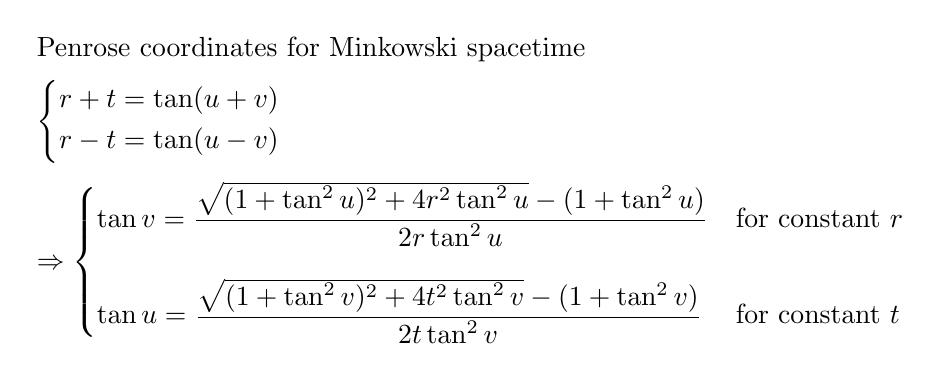
\begin{tikzpicture}[scale=1]
  \def\tu{\tan^2u} % shorthand
  \def\tv{\tan^2v} % shorthand
  \node[align=left] at (0,0)
    {Penrose coordinates for Minkowski spacetime\\[2mm]$
    \left\{\begin{aligned}
      r + t = \tan(u+v) \\
      r - t = \tan(u-v) \\
    \end{aligned}\right.$\\[2mm]$
    \Rightarrow\begin{cases}
      \tan v = \dfrac{\sqrt{(1+\tu)^2+4r^2\tu}-(1+\tu)}{2r\tu} & \text{for constant $r$} \\[5mm]
      \tan u = \dfrac{\sqrt{(1+\tv)^2+4t^2\tv}-(1+\tv)}{2t\tv} & \text{for constant $t$}
    \end{cases}$};
\end{tikzpicture}


% PENROSE DIAGRAM of Minkowski space - equidistant world lines
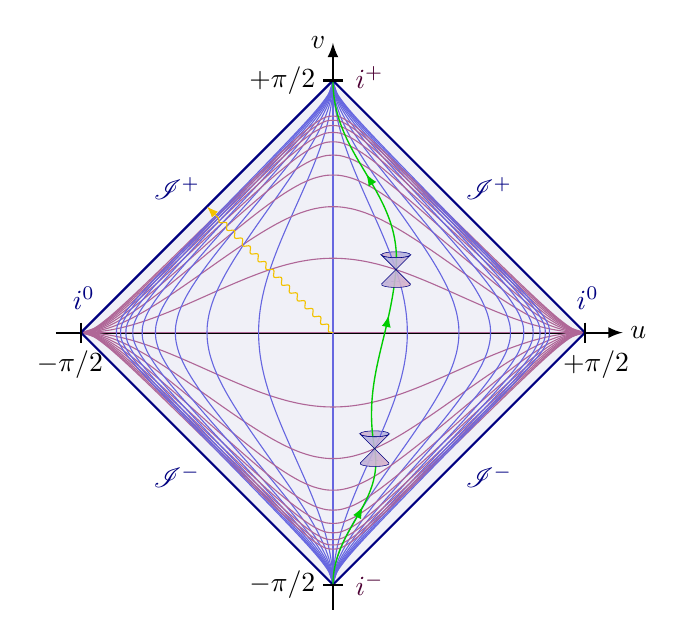
\begin{tikzpicture}[scale=3.2]
  \message{Penrose diagram (equidistant world lines)^^J}
  
  \def\Nlines{9} % number of world lines (at constant r/t)
  \def\d{0.5}
  \coordinate (O) at ( 0, 0); % center: origin (r,t) = (0,0)
  \coordinate (S) at ( 0,-1); % south: t=-infty, i-
  \coordinate (N) at ( 0, 1); % north: t=+infty, i+
  \coordinate (W) at (-1, 0); % east:  r=-infty, i0
  \coordinate (E) at ( 1, 0); % west:  r=+infty, i0
  \coordinate (X) at ({penroseu(\d,\d)},{penrosev(\d,\d)});
  \coordinate (X0) at ({penroseu(\d,-2*\d)},{penrosev(\d,-2*\d)});
  
  % AXES
  \fill[mylightblue] (N) -- (E) -- (S) -- (W) -- cycle;
  \draw[->,thick] (-1.1,0) -- (1.15,0) node[right=-1] {$u$};
  \draw[->,thick] (0,-1.1) -- (0,1.15) node[left=-1] {$v$};
  
  % INFINITY LABELS
  \node[right=1,above=1,mydarkblue] at (-1,0.04) {$i^0$};
  \node[right=1,above=1,mydarkblue] at (1,0.04) {$i^0$};
  \node[below=0,right=1,mydarkpurple] at (0.04,-1) {$i^-$};
  \node[above=1,right=1,mydarkpurple] at (0.04,1) {$i^+$};
  \node[mydarkblue,below left=-1] at (-0.5,-0.5) {$\calI^-$};
  \node[mydarkblue,above left=-1] at (-0.5,0.5) {$\calI^+$};
  \node[mydarkblue,above right=-1] at (0.5,0.5) {$\calI^+$};
  \node[mydarkblue,below right=-1] at (0.5,-0.5) {$\calI^-$};
  
  % LIGHT CONE BACK
  \coneback{X};
  \coneback{X0};
  
  % WORLD LINES
  \draw[world line] (N) -- (S);
  \draw[world line t] (W) -- (E);
  \message{Making world lines...^^J}
  \foreach \i [evaluate={\c=\i*\d;}] in {1,...,\Nlines}{
    \message{  Running i/N=\i/\Nlines, c=\c...^^J}
    \draw[world line t,samples=\Nsamples,smooth,variable=\x,domain=-1:1] % constant t
      plot(\x,{-penrose(\x*pi/2,\c)})
      plot(\x,{ penrose(\x*pi/2,\c)});
    \draw[world line,samples=\Nsamples,smooth,variable=\y,domain=-1:1] % constant r
      plot({-penrose(\y*pi/2,\c)},\y)
      plot({ penrose(\y*pi/2,\c)},\y);
  }
  \draw[thick,mydarkblue] (N) -- (E) -- (S) -- (W) -- cycle;
  
  % PARTICLE
  \draw[particle,decoration={markings,mark=at position 0.16 with {\arrow{latex}},
                                      mark=at position 0.53 with {\arrow{latex}},
                                      mark=at position 0.81 with {\arrow{latex}}},postaction={decorate}]
    (S) to[out=90,in=-80] (X0) to[out=100,in=-95] (X) to[out=85,in=-90] (N);
  
  % LIGHT CONE FRONT
  \conefront{X};
  \conefront{X0};
  
  % PHOTON
  \draw[->,photon] (O) -- (-0.5,0.5); %node[above=2,right=1] {photon};
  
  % TICKS
  \tick{W}{90} node[left=4,below=-1] {$-\pi/2$};
  \tick{E}{90} node[right=4,below=-1] {$+\pi/2$};
  \tick{S}{ 0} node[left=-1] {$-\pi/2$};
  \tick{N}{ 0} node[left=-1] {$+\pi/2$};
  
\end{tikzpicture}


% PENROSE DIAGRAM of Minkowski space
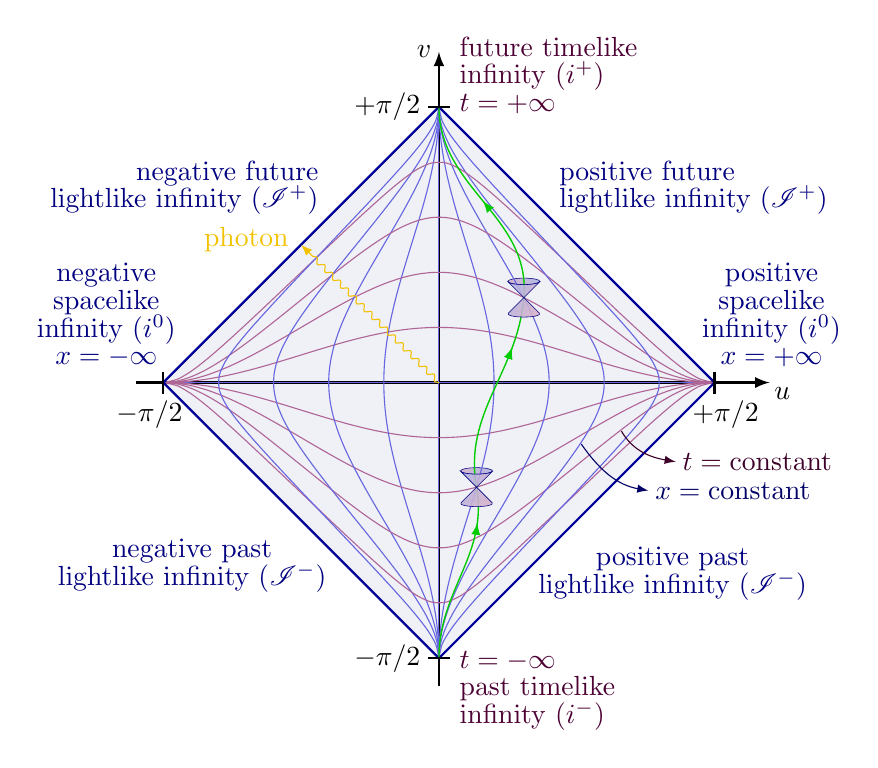
\begin{tikzpicture}[scale=3.5]
  \message{Penrose diagram^^J}
  
  \def\Nlines{4} % number of world lines (at constant r/t)
  \def\ta{tan(90*1.0/(\Nlines+1))} % constant r/t value 1
  \def\tb{tan(90*2.0/(\Nlines+1))} % constant r/t value 2
  \coordinate (O) at ( 0, 0); % center: origin (r,t) = (0,0)
  \coordinate (S) at ( 0,-1); % south: t=-infty, i-
  \coordinate (N) at ( 0, 1); % north: t=+infty, i+
  \coordinate (W) at (-1, 0); % east:  r=-infty, i0
  \coordinate (E) at ( 1, 0); % west:  r=+infty, i0
  \coordinate (X) at ({penroseu(\tb,\tb)},{penrosev(\tb,\tb)});
  \coordinate (X0) at ({penroseu(\ta,-\tb)},{penrosev(\ta,-\tb)});
  
  % AXES
  \fill[mylightblue] (N) -- (E) -- (S) -- (W) -- cycle;
  \draw[->,thick] (-1.1,0) -- (1.2,0) node[below right=-2] {$u$};
  \draw[->,thick] (0,-1.1) -- (0,1.2) node[left=-1] {$v$};
  
  % INFINITY LABELS
  \node[right=6,above left=-2,mydarkblue,align=center] at (-1,0.04)
    {negative\\[-2]spacelike\\[-2]infinity ($i^0$)\\[-2]$x=-\infty$};
  \node[left=6,above right=-2,mydarkblue,align=center] at (1,0.04)
    {positive\\[-2]spacelike\\[-2]infinity ($i^0$)\\[-2]$x=+\infty$};
  \node[above=6,below right=0,mydarkpurple,align=left] at (0.04,-1)
    {$t=-\infty$\\[-2]past timelike\\[-2]infinity ($i^-$)};
  \node[below=6,above right=0,mydarkpurple,align=left] at (0.04,1)
    {future timelike\\[-2]infinity ($i^+$)\\[-2]$t=+\infty$};
  \node[mydarkblue,above right,align=left] at (55:0.7)
    {positive future\\[-2]lightlike infinity ($\calI^+$)};
  \node[mydarkblue,below right,align=center] at (-60:0.65)
    {positive past\\[-2]lightlike infinity ($\calI^-$)};
  \node[mydarkblue,above left,align=right] at (125:0.7)
    {negative future\\[-2]lightlike infinity ($\calI^+$)};
  \node[mydarkblue,below left,align=center] at (-125:0.65)
    {negative past\\[-2]lightlike infinity ($\calI^-$)};
  
  % CONE BACK
  \coneback{X};
  \coneback{X0};
  
  % WORLD LINES
  \draw[world line] (N) -- (S);
  \draw[world line] (W) -- (E);
  \message{Making world lines...^^J}
  \foreach \i [evaluate={\c=\i/(\Nlines+1); \ct=tan(90*\c);}] in {1,...,\Nlines}{
    \message{  Running i/N=\i/\Nlines, c=\c, tan(90*\c)=\ct...^^J}
    \draw[world line t,samples=\Nsamples,smooth,variable=\t,domain=-1:1] % constant t
      plot(\t,{-penrose(\t*pi/2,\ct)})
      plot(\t,{ penrose(\t*pi/2,\ct)});
    \draw[world line,samples=\Nsamples,smooth,variable=\x,domain=-1:1] % constant r
      plot({-penrose(\x*pi/2,\ct)},\x)
      plot({ penrose(\x*pi/2,\ct)},\x);
  }
  \draw[thick,blue!60!black] (N) -- (E) -- (S) -- (W) -- cycle;
  
  % CONSTANT
  \draw[->,mydarkpurple!80!black,shorten <=0.4] % constant r
    (0.66,{-penrose(0.66*pi/2,tan(90*3/(\Nlines+1)))}) to[out=-60,in=170]++ (-30:0.23)
    node[right=-1] {$t=\text{constant}$};
  \draw[->,mydarkblue!80!black,shorten <=0.4] % constant t
    ({penrose(-0.22*pi/2,tan(90*3/(\Nlines+1)))},-0.22) to[out=-55,in=170]++ (-35:0.3)
    node[right=-1] {$x=\text{constant}$};
  
  % PARTICLE
  \draw[particle,decoration={markings,mark=at position 0.24 with {\arrow{latex}},
                                      mark=at position 0.55 with {\arrow{latex}},
                                      mark=at position 0.82 with {\arrow{latex}}},postaction={decorate}]
    (S) to[out=90,in=-80] (X0) to[out=100,in=-95] (X) to[out=85,in=-90] (N);
  
  % LIGHT CONE FRONT
  \conefront{X};
  \conefront{X0};
  
  % PHOTON
  \draw[->,photon] (O) -- (-0.5,0.5) node[above=2,left=1] {photon};
  
  % TICKS
  \tick{W}{90} node[left=5,below=-1] {$-\pi/2$};
  \tick{E}{90} node[right=4,below=-1] {$+\pi/2$};
  \tick{S}{ 0} node[left=-1] {$-\pi/2$};
  \tick{N}{ 0} node[left=-1] {$+\pi/2$};
  
\end{tikzpicture}


% PENROSE DIAGRAM of Minkowski space - radius r
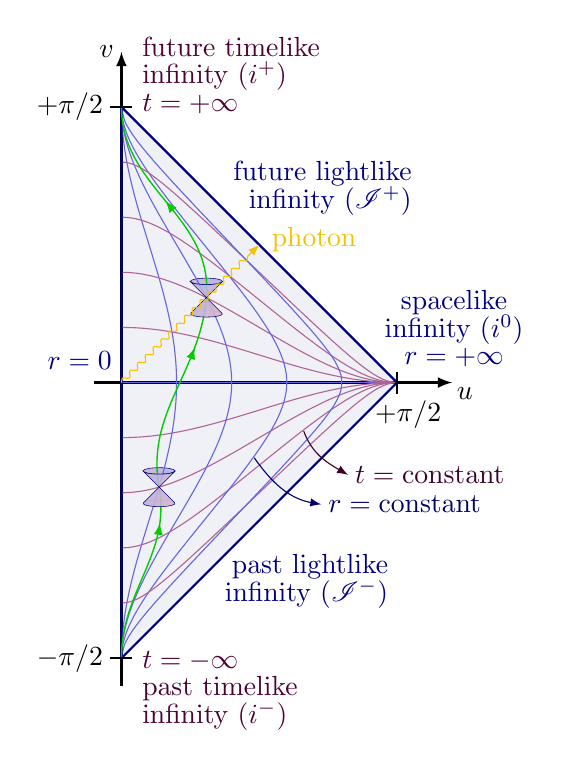
\begin{tikzpicture}[scale=3.5]
  \message{Penrose diagram (radius r)^^J}
  
  \def\Nlines{4} % number of world lines (at constant r/t)
  \def\ta{tan(90*1.0/(\Nlines+1))} % constant r/t value 1
  \def\tb{tan(90*2.0/(\Nlines+1))} % constant r/t value 2
  \coordinate (O) at ( 0, 0); % center: origin (r,t) = (0,0)
  \coordinate (S) at ( 0,-1); % south: t=-infty, i-
  \coordinate (N) at ( 0, 1); % north: t=+infty, i+
  \coordinate (E) at ( 1, 0); % east:  r=+infty, i0
  \coordinate (X) at ({penroseu(\tb,\tb)},{penrosev(\tb,\tb)});
  \coordinate (X0) at ({penroseu(\ta,-\tb)},{penrosev(\ta,-\tb)});
  
  % AXES
  \fill[mylightblue] (N) -- (E) -- (S) -- cycle;
  \draw[->,thick] (-0.1,0) -- (1.2,0) node[below right=-2] {$u$};
  \draw[->,thick] (0,-1.1) -- (0,1.2) node[left=-1] {$v$};
  
  % INFINITY LABELS
  \node[above=1,above left=0,mydarkblue,align=center] at (O)
    {$r=0$};
  \node[left=6,above right=-2,mydarkblue,align=center] at (1,0.04)
    {spacelike\\[-2]infinity ($i^0$)\\[-2]$r=+\infty$};
  \node[above=6,below right=0,mydarkpurple,align=left] at (0.04,-1)
    {$t=-\infty$\\[-2]past timelike\\[-2]infinity ($i^-$)};
  \node[below=6,above right=0,mydarkpurple,align=left] at (0.04,1)
    {future timelike\\[-2]infinity ($i^+$)\\[-2]$t=+\infty$};
  \node[mydarkblue,above right,align=right] at (57:0.68)
    {future lightlike\\[-2]infinity ($\calI^+$)};
  \node[mydarkblue,below right,align=right] at (-60:0.68)
    {past lightlike\\[-2]infinity ($\calI^-$)};
  
  % CONE BACK
  \coneback{X};
  \coneback{X0};
  
  % WORLD LINES
  \draw[world line] (N) -- (S);
  \draw[world line] (O) -- (E);
  \message{Making world lines...^^J}
  \foreach \i [evaluate={\c=\i/(\Nlines+1); \ct=tan(90*\c);}] in {1,...,\Nlines}{
    \message{  Running i/N=\i/\Nlines, c=\c, tan(90*\c)=\ct...^^J}
    \draw[world line t,samples=\Nsamples,smooth,variable=\t,domain=0.001:1] % constant t
      plot(\t,{-penrose(\t*pi/2,\ct)})
      plot(\t,{ penrose(\t*pi/2,\ct)});
    \draw[world line,samples=\Nsamples,smooth,variable=\r,domain=-1:1] % constant r
      plot({penrose(\r*pi/2,\ct)},\r);
  }
  \draw[thick,mydarkblue] (N) -- (E) -- (S) -- cycle;
  
  % CONSTANT
  \draw[->,mydarkpurple!80!black,shorten <=0.4] % constant r
    (0.66,{-penrose(0.66*pi/2,tan(90*3/(\Nlines+1)))}) to[out=-70,in=150]++ (-45:0.23)
    node[right=-1] {$t=\text{constant}$};
  \draw[->,mydarkblue!80!black,shorten <=0.4] % constant t
    ({penrose(-0.27*pi/2,tan(90*3/(\Nlines+1)))},-0.27) to[out=-55,in=170]++ (-35:0.3)
    node[right=-1] {$r=\text{constant}$};
  
  % PARTICLE
  \draw[particle,decoration={markings,mark=at position 0.24 with {\arrow{latex}},
                                      mark=at position 0.55 with {\arrow{latex}},
                                      mark=at position 0.82 with {\arrow{latex}}},postaction={decorate}]
    (S) to[out=90,in=-80] (X0) to[out=100,in=-95] (X) to[out=85,in=-90] (N);
  
  % LIGHT CONE FRONT
  \conefront{X};
  \conefront{X0};
  
  % PHOTON
  \draw[->,photon] (O) -- (0.5,0.5) node[above=2,right=1] {photon};
  
  % TICKS
  \tick{E}{90} node[right=4,below=-1] {$+\pi/2$};
  \tick{S}{ 0} node[left=-1] {$-\pi/2$};
  \tick{N}{ 0} node[left=-1] {$+\pi/2$};
  
\end{tikzpicture}


% PENROSE COORDINATES for Kruskal-Szekeres coordinates
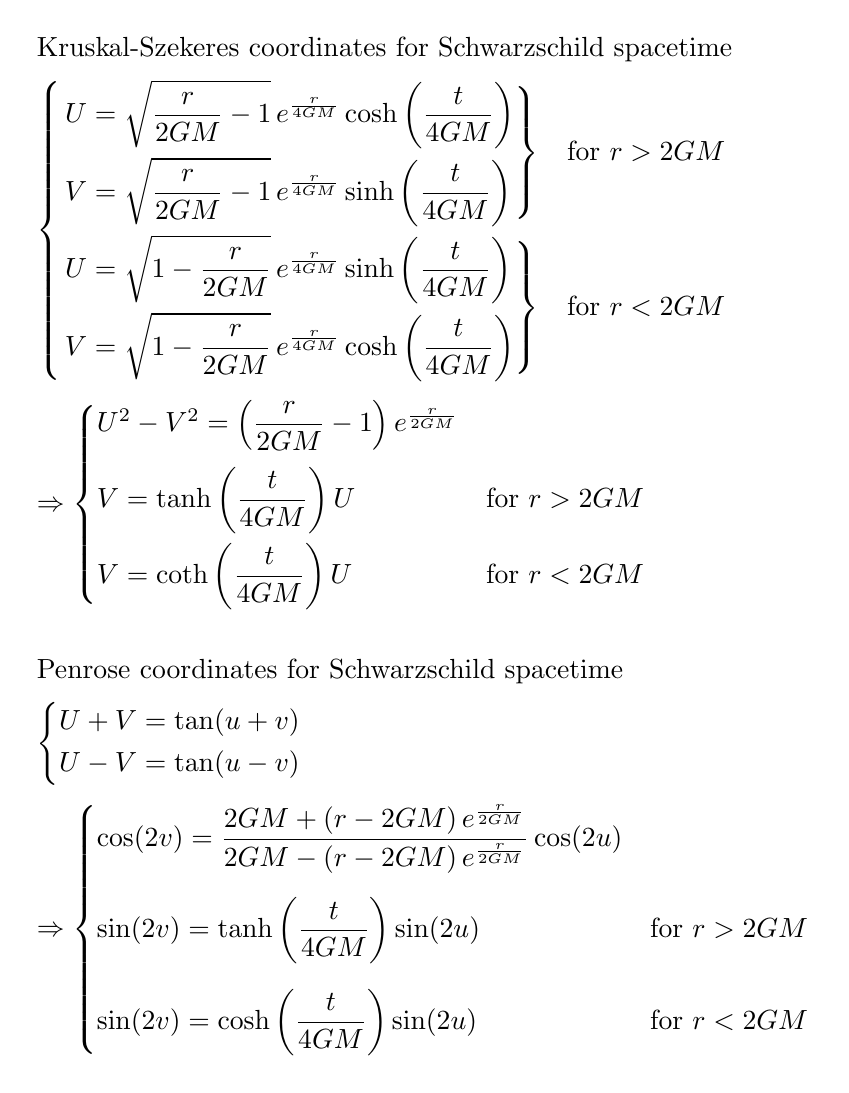
\begin{tikzpicture}[scale=1]
  \def\tu{\tan^2u} % shorthand
  \def\tv{\tan^2v} % shorthand
  \node[align=left] at (0,0) {
    Kruskal-Szekeres coordinates for Schwarzschild spacetime\\[2mm]
    $\displaystyle
    \begin{cases}
      \left.\begin{aligned}
        U &= \sqrt{\frac{r}{2GM}-1}\,e^{\frac{r}{4GM}}\cosh\left(\frac{t}{4GM}\right) \\
        V &= \sqrt{\frac{r}{2GM}-1}\,e^{\frac{r}{4GM}}\sinh\left(\frac{t}{4GM}\right) \\
      \end{aligned}\right\} &\text{for $r>2GM$} \\[8mm]
      \left.\begin{aligned}
        U &= \sqrt{1-\frac{r}{2GM}}\,e^{\frac{r}{4GM}}\sinh\left(\frac{t}{4GM}\right) \\
        V &= \sqrt{1-\frac{r}{2GM}}\,e^{\frac{r}{4GM}}\cosh\left(\frac{t}{4GM}\right) \\
      \end{aligned}\right\} &\text{for $r<2GM$}
    \end{cases}$\\[2mm]
    $\displaystyle
    \Rightarrow\begin{cases}
      U^2 - V^2 = \left(\dfrac{r}{2GM}-1\right)e^{\frac{r}{2GM}} \\[3mm]
      V = \tanh\left(\dfrac{t}{4GM}\right)U & \text{for $r>2GM$} \\[3mm]
      V = \coth\left(\dfrac{t}{4GM}\right)U & \text{for $r<2GM$}
    \end{cases}$\\[6mm]
    Penrose coordinates for Schwarzschild spacetime\\[2mm]$
    \left\{\begin{aligned}
      U + V = \tan(u+v) \\
      U - V = \tan(u-v) \\
    \end{aligned}\right.$\\[2mm]
    $\displaystyle
    \Rightarrow\begin{cases}
      \cos(2v) = \dfrac{2GM+\left(r-2GM\right)e^{\frac{r}{2GM}}}
                       {2GM-\left(r-2GM\right)e^{\frac{r}{2GM}}}
                 \cos(2u) \\[5mm]
      \sin(2v) = \tanh\left(\dfrac{t}{4GM}\right)\sin(2u) & \text{for $r>2GM$} \\[5mm]
      \sin(2v) = \cosh\left(\dfrac{t}{4GM}\right)\sin(2u) & \text{for $r<2GM$}
    \end{cases}$};
\end{tikzpicture}


% PENROSE DIAGRAM of a Schwarzschild black hole
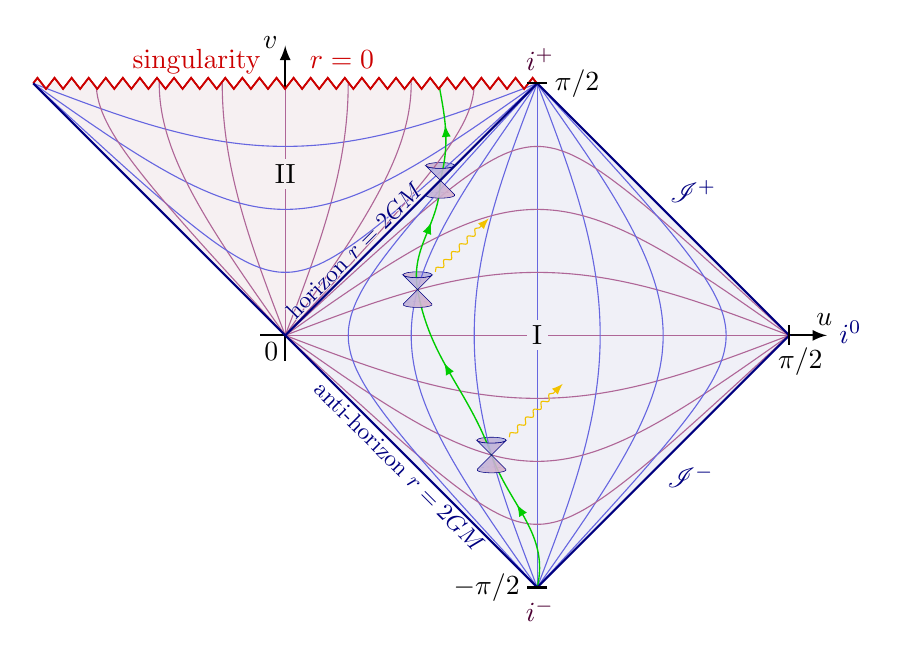
\begin{tikzpicture}[scale=3.2]
  \message{Extended Penrose diagram: Schwarzschild black hole^^J}
  
  \def\R{0.08} % size lightcone
  \def\Nlines{3} % number of world lines (at constant r/t)
  \pgfmathsetmacro\ta{1/sin(90*1/(\Nlines+1))} % constant r/t value 1
  \pgfmathsetmacro\tb{sin(90*2/(\Nlines+1))}   % constant r/t value 2
  \pgfmathsetmacro\tc{1/sin(90*2/(\Nlines+1))} % constant r/t value 3
  \pgfmathsetmacro\td{sin(90*1/(\Nlines+1))}   % constant r/t value 4
  \coordinate (-O) at (-1, 0); % center III: origin (r,t) = (0,0)
  \coordinate (-N) at (-1, 1); % north III: t=+infty, i+
  \coordinate (O)  at ( 1, 0); % center I: origin (r,t) = (0,0)
  \coordinate (S)  at ( 1,-1); % south I: t=-infty, i-
  \coordinate (N)  at ( 1, 1); % north I: t=+infty, i+
  \coordinate (E)  at ( 2, 0); % east I:  r=-infty, i0
  \coordinate (W)  at ( 0, 0); % west I:  r=+infty, i0
  \coordinate (B)  at ( 0,-1); % singularity bottom
  \coordinate (X0) at ({asin(sqrt((\ta^2-1)/(\ta^2-\tb^2)))/90},
                       {-acos(\ta*sqrt((1-\tb^2)/(\ta^2-\tb^2)))/90}); % particle 1
  \coordinate (X1) at ({asin(sqrt((\tc^2-1)/(\tc^2-\td^2)))/90},
                       {acos(\tc*sqrt((1-\td^2)/(\tc^2-\td^2)))/90}); % particle 2
  \coordinate (X2) at (45:0.87); % particle falling in BH horizon
  \coordinate (X3) at (0.60,1.05); % particle falling in BH singularity
  
  % AXES
  \draw[->,thick] (0,-0.1) -- (0,1.15) node[above=1,left=-1] {$v$};
  \draw[->,thick] (-0.1,0) -- (2.15,0) node[left=1,above=0] {$u$};
  
  \begin{scope}
    
    % CLIP to fill inside zigzag lines
    \clip[decorate,decoration={zigzag,amplitude=2,segment length=6.17}]
      (-N) -- (N) --++ (1.1,0.1) |-++ (-3.1,-2.3) -- cycle;
    
    % REGIONS FILLS
    \fill[mylightpurple] (-N) |-++ (2,0.1) -- (N) -- (W) -- cycle;
    \fill[mylightblue] (N) -- (E) -- (S) -- (W) -- cycle;
    
    % CONE BACK
    \coneback{X0};
    \coneback{X1};
    \coneback{X2};
    
    % WORLD LINES
    \draw[world line] (N) -- (S);
    \draw[world line t] (W) -- (E) (W) -- (0,1.1);
    \message{Making world lines...^^J}
    \foreach \i [evaluate={\c=\i/(\Nlines+1); \cs=sin(90*\c);}] in {1,...,\Nlines}{
      \message{  Running i/N=\i/\Nlines, c=\c, cs=\cs...^^J}
      \draw[world line t,samples=\Nsamples,smooth,variable=\x,domain=0:2] % region I, constant t
        plot(\x,{-kruskal(\x*pi/4,\cs)})
        plot(\x,{ kruskal(\x*pi/4,\cs)});
      \draw[world line,samples=\Nsamples,smooth,variable=\y,domain=0:2] % region I, constant r
        plot({1-kruskal(\y*pi/4,\cs)},\y-1)
        plot({1+kruskal(\y*pi/4,\cs)},\y-1);
      \draw[world line,samples=\Nsamples,smooth,variable=\x,domain=0:2] % region II, constant r
        plot(\x-1,{1-kruskal(\x*pi/4,\cs)});
      \draw[world line t,samples=\Nsamples,smooth,variable=\y,domain=0:1.05] % region II constant t
        plot({-kruskal(\y*pi/4,\cs)},\y)
        plot({ kruskal(\y*pi/4,\cs)},\y);
    }
    
    % PARTICLE WORLD LINE
    \draw[particle,decoration={markings,mark=at position 0.16 with {\arrow{latex}},
                                        mark=at position 0.45 with {\arrow{latex}},
                                        mark=at position 0.72 with {\arrow{latex}},
                                        mark=at position 0.90 with {\arrow{latex}}},postaction={decorate}]
      (S) to[out=77,in=-70] (X0) to[out=110,in=-80] (X1)
          to[out=100,in=-90] (X2) to[out=75,in=-80] (X3);
  
  \end{scope}
  
  % LIGHT CONE FRONT
  \conefront{X0};
  \conefront{X1};
  \conefront{X2};
  
  % ESCAPING PHOTONS
  \draw[photon] (X0) ++ (45:0.1) --++ (45:0.3);
  \draw[photon] (X1) ++ (45:0.1) --++ (45:0.3);
  
  % REGIONS
  \node[fill=mylightblue,inner sep=2] at (O) {I};
  \node[fill=mylightpurple,inner sep=2] at (0,0.64) {II};
  
  % BOUNDARIES
  \draw[singularity] (-N) -- node[pos=0.46,above left=-2] {\strut singularity} (N);
  \draw[singularity] (-N) -- node[pos=0.54,above right=-2] {\strut $r=0$} (N);
  \path (S) -- (W) node[mydarkblue,pos=0.50,below=-2.5,rotate=-45,scale=0.85]
    {anti-horizon $r=2GM$};
  \path (W) -- (N) node[mydarkblue,pos=0.32,above=-2.5,rotate=45,scale=0.85]
    {\contour{mylightpurple}{horizon $r=2GM$}};
  \draw[thick,mydarkblue] (N) -- (E) -- (S) --  (W) -- cycle;
  \draw[thick,mydarkblue] (W) -- (-N);
  
  % TICKS
  \node[below left=-1] at (W) {$0$};
  \tick{E}{90} node[right=4,below=-3] {$\pi/2$};
  \tick{S}{0} node[left=-1] {$-\pi/2$};
  \tick{N}{180} node[right=-1] {$\pi/2$};
  
  % INFINITY LABELS
  \node[above=1,right=1,mydarkblue] at (2.15,0) {$i^0$};
  \node[right=1,below=1,mydarkpurple] at (S) {$i^-$};
  \node[right=1,above=1,mydarkpurple] at (N) {$i^+$};
  \node[mydarkblue,above right=-1] at (1.5,0.5) {$\calI^+$};
  \node[mydarkblue,below right=-2] at (1.5,-0.5) {$\calI^-$};
  
\end{tikzpicture}


% EXTENDED PENROSE DIAGRAM of a Schwarzschild black hole
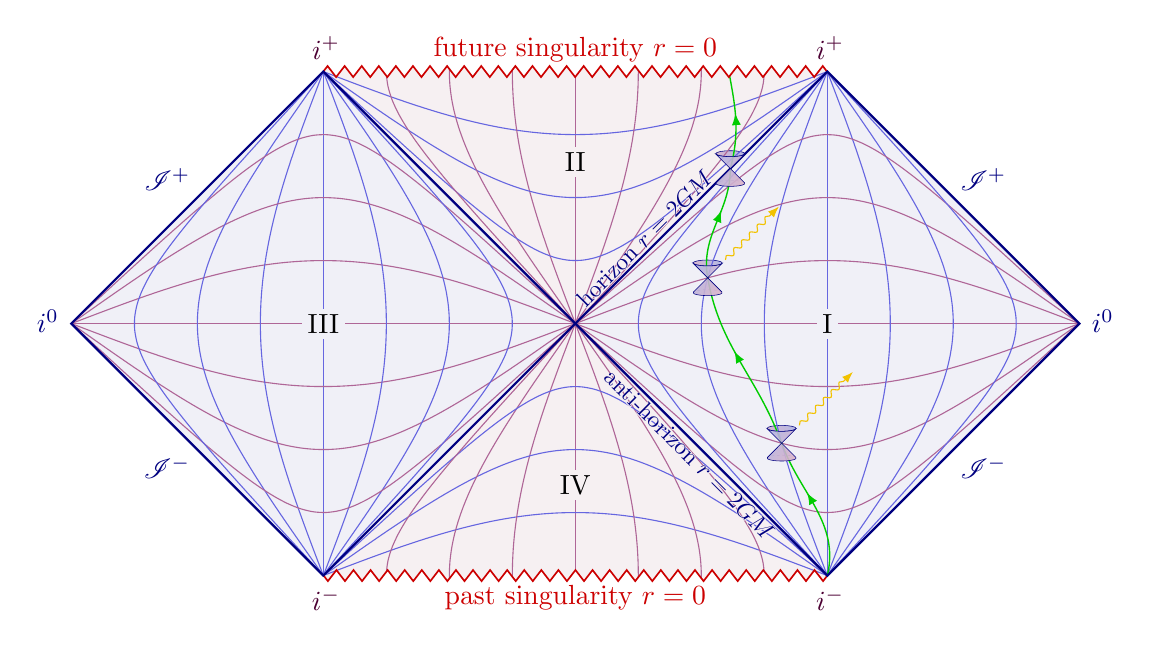
\begin{tikzpicture}[scale=3.2]
  \message{Extended Penrose diagram: Schwarzschild black hole^^J}
  
  \def\R{0.08} % size lightcone
  \def\Nlines{3} % number of world lines (at constant r/t)
  \pgfmathsetmacro\ta{1/sin(90*1/(\Nlines+1))} % constant r/t value 1
  \pgfmathsetmacro\tb{sin(90*2/(\Nlines+1))}   % constant r/t value 2
  \pgfmathsetmacro\tc{1/sin(90*2/(\Nlines+1))} % constant r/t value 3
  \pgfmathsetmacro\td{sin(90*1/(\Nlines+1))}   % constant r/t value 4
  \coordinate (-O) at (-1, 0); % center III: origin (r,t) = (0,0)
  \coordinate (-S) at (-1,-1); % south III: t=-infty, i-
  \coordinate (-N) at (-1, 1); % north III: t=+infty, i+
  \coordinate (-W) at (-2, 0); % east III:  r=-infty, i0
  \coordinate (-E) at ( 0, 0); % west III:  r=+infty, i0
  \coordinate (O)  at ( 1, 0); % center I: origin (r,t) = (0,0)
  \coordinate (S)  at ( 1,-1); % south I: t=-infty, i-
  \coordinate (N)  at ( 1, 1); % north I: t=+infty, i+
  \coordinate (E)  at ( 2, 0); % east I:  r=-infty, i0
  \coordinate (W)  at ( 0, 0); % west I:  r=+infty, i0
  \coordinate (B)  at ( 0,-1); % singularity bottom
  \coordinate (T)  at ( 0, 1); % singularity top
  \coordinate (X0) at ({asin(sqrt((\ta^2-1)/(\ta^2-\tb^2)))/90},
                       {-acos(\ta*sqrt((1-\tb^2)/(\ta^2-\tb^2)))/90}); % particle 1
  \coordinate (X1) at ({asin(sqrt((\tc^2-1)/(\tc^2-\td^2)))/90},
                       {acos(\tc*sqrt((1-\td^2)/(\tc^2-\td^2)))/90}); % particle 2
  \coordinate (X2) at (45:0.87); % particle falling in BH horizon
  \coordinate (X3) at (0.60,1.05); % particle falling in BH singularity
  
  \begin{scope}
    
    % CLIP to fill inside zigzag lines
    \clip[decorate,decoration={zigzag,amplitude=2,segment length=6.17}]
      (S) -- (-S) --++ (-1.1,-0.1) |-++ (4.2,2.2) |- cycle;
    \clip[decorate,decoration={zigzag,amplitude=2,segment length=6.17}]
      (-N) -- (N) --++ (1.1,0.1) |-++ (-4.2,-2.2) |- cycle;
    
    % REGIONS FILLS
    \fill[mylightpurple] (-N) |-++ (2,0.1) -- (N) -- (-S) -- (S) -- cycle;
    \fill[mylightpurple] (-S) |-++ (2,-0.1) -- (S) -- (-N) -- (N) -- cycle;
    
    \fill[mylightblue] (-N) -- (-E) -- (-S) -- (-W) -- cycle;
    \fill[mylightblue] (N) -- (E) -- (S) -- (W) -- cycle;
    
    % CONE BACK
    \coneback{X0};
    \coneback{X1};
    \coneback{X2};
    
    % WORLD LINES
    \draw[world line] (-N) -- (-S) (N) -- (S);
    \draw[world line t] (-W) -- (-E) (W) -- (E) (0,-1.1) -- (0,1.1);
    \message{Making world lines...^^J}
    \foreach \i [evaluate={\c=\i/(\Nlines+1); \cs=sin(90*\c);}] in {1,...,\Nlines}{
      \message{  Running i/N=\i/\Nlines, c=\c, cs=\cs...^^J}
      \draw[world line t,samples=2*\Nsamples,smooth,variable=\x,domain=-2:2] % region I/III, constant t
        plot(\x,{-kruskal(\x*pi/4,\cs)})
        plot(\x,{ kruskal(\x*pi/4,\cs)});
      \draw[world line,samples=\Nsamples,smooth,variable=\y,domain=0:2] % region I/III, constant r
        plot({-1-kruskal(\y*pi/4,\cs)},\y-1)
        plot({-1+kruskal(\y*pi/4,\cs)},\y-1)
        plot({1-kruskal(\y*pi/4,\cs)},\y-1)
        plot({1+kruskal(\y*pi/4,\cs)},\y-1);
      \draw[world line,samples=\Nsamples,smooth,variable=\x,domain=0:2] % region II/IV, constant r
        plot(\x-1,{kruskal(\x*pi/4,\cs)-1})
        plot(\x-1,{1-kruskal(\x*pi/4,\cs)});
      \draw[world line t,samples=\Nsamples,smooth,variable=\y,domain=-1.05:1.05] % region II/IV constant t
        plot({-kruskal(\y*pi/4,\cs)},\y)
        plot({ kruskal(\y*pi/4,\cs)},\y);
    }
    
    % PARTICLE WORLD LINE
    \draw[particle,decoration={markings,mark=at position 0.16 with {\arrow{latex}},
                                        mark=at position 0.45 with {\arrow{latex}},
                                        mark=at position 0.72 with {\arrow{latex}},
                                        mark=at position 0.90 with {\arrow{latex}}},postaction={decorate}]
      (S) to[out=77,in=-70] (X0) to[out=110,in=-80] (X1)
          to[out=100,in=-90] (X2) to[out=75,in=-80] (X3);
    
  \end{scope}
  
  % BOUNDARIES
  \draw[singularity] (-N) -- node[above] {future singularity $r=0$} (N);
  \draw[singularity] (S) -- node[below] {past singularity $r=0$} (-S);
  \path (S) -- (W) node[mydarkblue,pos=0.50,below=-2.5,rotate=-45,scale=0.85]
    {\contour{mylightpurple}{anti-horizon $r=2GM$}};
  \path (W) -- (N) node[mydarkblue,pos=0.32,above=-2.5,rotate=45,scale=0.85]
    {\contour{mylightpurple}{horizon $r=2GM$}};
  \draw[thick,mydarkblue] (-N) -- (-E) -- (-S) -- (-W) -- cycle;
  \draw[thick,mydarkblue] (N) -- (E) -- (S) -- (W) -- cycle;
  
  % REGIONS
  \node[fill=mylightblue,inner sep=2] at (-O) {III};
  \node[fill=mylightblue,inner sep=2] at (O) {I};
  \node[fill=mylightpurple,inner sep=2] at (0,0.64) {II};
  \node[fill=mylightpurple,inner sep=2] at (0,-0.64) {IV};
  
  % INFINITY LABELS
  \node[above=1,left=1,mydarkblue] at (-2,0) {$i^0$};
  \node[above=1,right=1,mydarkblue] at (2,0) {$i^0$};
  \node[right=1,below=1,mydarkpurple] at (-S) {$i^-$};
  \node[right=1,above=1,mydarkpurple] at (-N) {$i^+$};
  \node[right=1,below=1,mydarkpurple] at (S) {$i^-$};
  \node[right=1,above=1,mydarkpurple] at (N) {$i^+$};
  \node[mydarkblue,below left=-1] at (-1.5,-0.5) {$\calI^-$};
  \node[mydarkblue,above left=-1] at (-1.5,0.5) {$\calI^+$};
  \node[mydarkblue,above right=-1] at (1.5,0.5) {$\calI^+$};
  \node[mydarkblue,below right=-1] at (1.5,-0.5) {$\calI^-$};
  
  % LIGHT CONE FRONT
  \conefront{X0};
  \conefront{X1};
  \conefront{X2};
  
  % ESCAPING PHOTONS
  \draw[photon] (X0) ++ (45:0.1) --++ (45:0.3);
  \draw[photon] (X1) ++ (45:0.1) --++ (45:0.3);
  
\end{tikzpicture}


\end{document}